\documentclass[letterpaper]{article}

\usepackage[english]{babel}
\usepackage[utf8]{inputenc}
\usepackage{amsmath}
\usepackage{graphicx}
\usepackage[colorinlistoftodos]{todonotes}
\usepackage[]{algorithm2e}
\usepackage{listings}
\usepackage{hyperref}
\usepackage{float}
\usepackage{afterpage}

\newcommand\blankpage{%
	\null
	\thispagestyle{empty}%
	\addtocounter{page}{-1}%
	\newpage}

\title{CSCE 689: Cloud Computing Project I}
\author{Aryan Sharma (UIN: 326006767)}

\date{\today}

\begin{document}
%\maketitle

%\afterpage{\blankpage}
%\newpage

\begin{titlepage}
	\centering
	%\includegraphics[width=0.15\textwidth]{example-image-1x1}\par\vspace{1cm}
	{\scshape\LARGE Texas A\&M University \par}
	\vspace{1cm}
	{\scshape\Large CSCE 689: Cloud Computing Project I\par}
	\vspace{1.5cm}
	{\huge\bfseries OpenStack v0.2\par}
	\vspace{2cm}
	{\Large Aryan Sharma \par}
	{\normalsize UIN: 326006767 | aryans@tamu.edu\par}
	\vfill
	Implemented in C++
	\vfill
	
	% Bottom of the page
	{\large \today\par}
\end{titlepage}

\tableofcontents
%\afterpage{\blankpage}

\newpage

\section{Project Information}
\label{sec:introduction}

This project implements a simple version of OpenStack in two steps: P0 and P1. \textbf{The github link for the code is: }

\vspace{1em}	
	\texttt{https://github.tamu.edu/aryans/689-18-a/tree/master/P1}
\vspace{1em}

The code has been written in C++ and it is contained within \texttt{AggieStack.cpp, AggieStack.h, Main.cpp, MakeFile}. Following are the overall functions of the files:

\begin{enumerate}
	\item \texttt{AggieStack.h}: It is the header file of the AggieStack.cpp file and contains the class definitions, global variables and the inline functions used.
	\item \texttt{AggieStack.cpp}: Contains the class function implementations.
	\item \texttt{Main.cpp}: It is the main driver of the AggieStack v0.2. It contains the CLI implementations and the \texttt{main()} function.
	\item \texttt{MakeFile}: Contains the direction as to how to run the program. 
	\item \texttt{aggiestack-log-date.txt}: Contains the log updates. 
\end{enumerate}

The time spent to complete this project was three days for v0.1 and about seven days for v0.2. It was done over a month in short bursts. Note that not all v0.1 commands are not suported in the v0.2 versions due to changes in the config files. To get the v0.1 the code has to be switched back to a prior git commit. However the CLI is missing in that git version. 

\section{Steps to run the code}

\begin{enumerate}
	\item \texttt{make clean}: to remove all the object files and previous logs.
	\item \texttt{make}: to compile the program. This would generate the executable file \textit{Main}.
	\item \texttt{./Main}: to run the program. This is a helper mode where it prints how to use this binary. 
	\item \texttt{./Main command\_file}: to run the program with a text files containing the commands. Any command that begins with \texttt{\#} are treated as comments and are ignored. 
	\item \texttt{./Main -I}: to run the program in an interactive mode. Commands can be issued now one by one and the output can be observed in the command line. 
	\item \texttt{./Main -help}: to get the instructions to run the program.
\end{enumerate}



\section{Command Line Interface Design}

A list of commands can be run using a file. The method to run it has been described above as: \texttt{./Main commands.txt}. The command line interface is reached by \texttt{./Main -I} or \texttt{./Main -i}. Some initial instructions can be fetched by \texttt{./Main -help}. A screenshot below explains this. 

\begin{figure} [H]
	\centering
	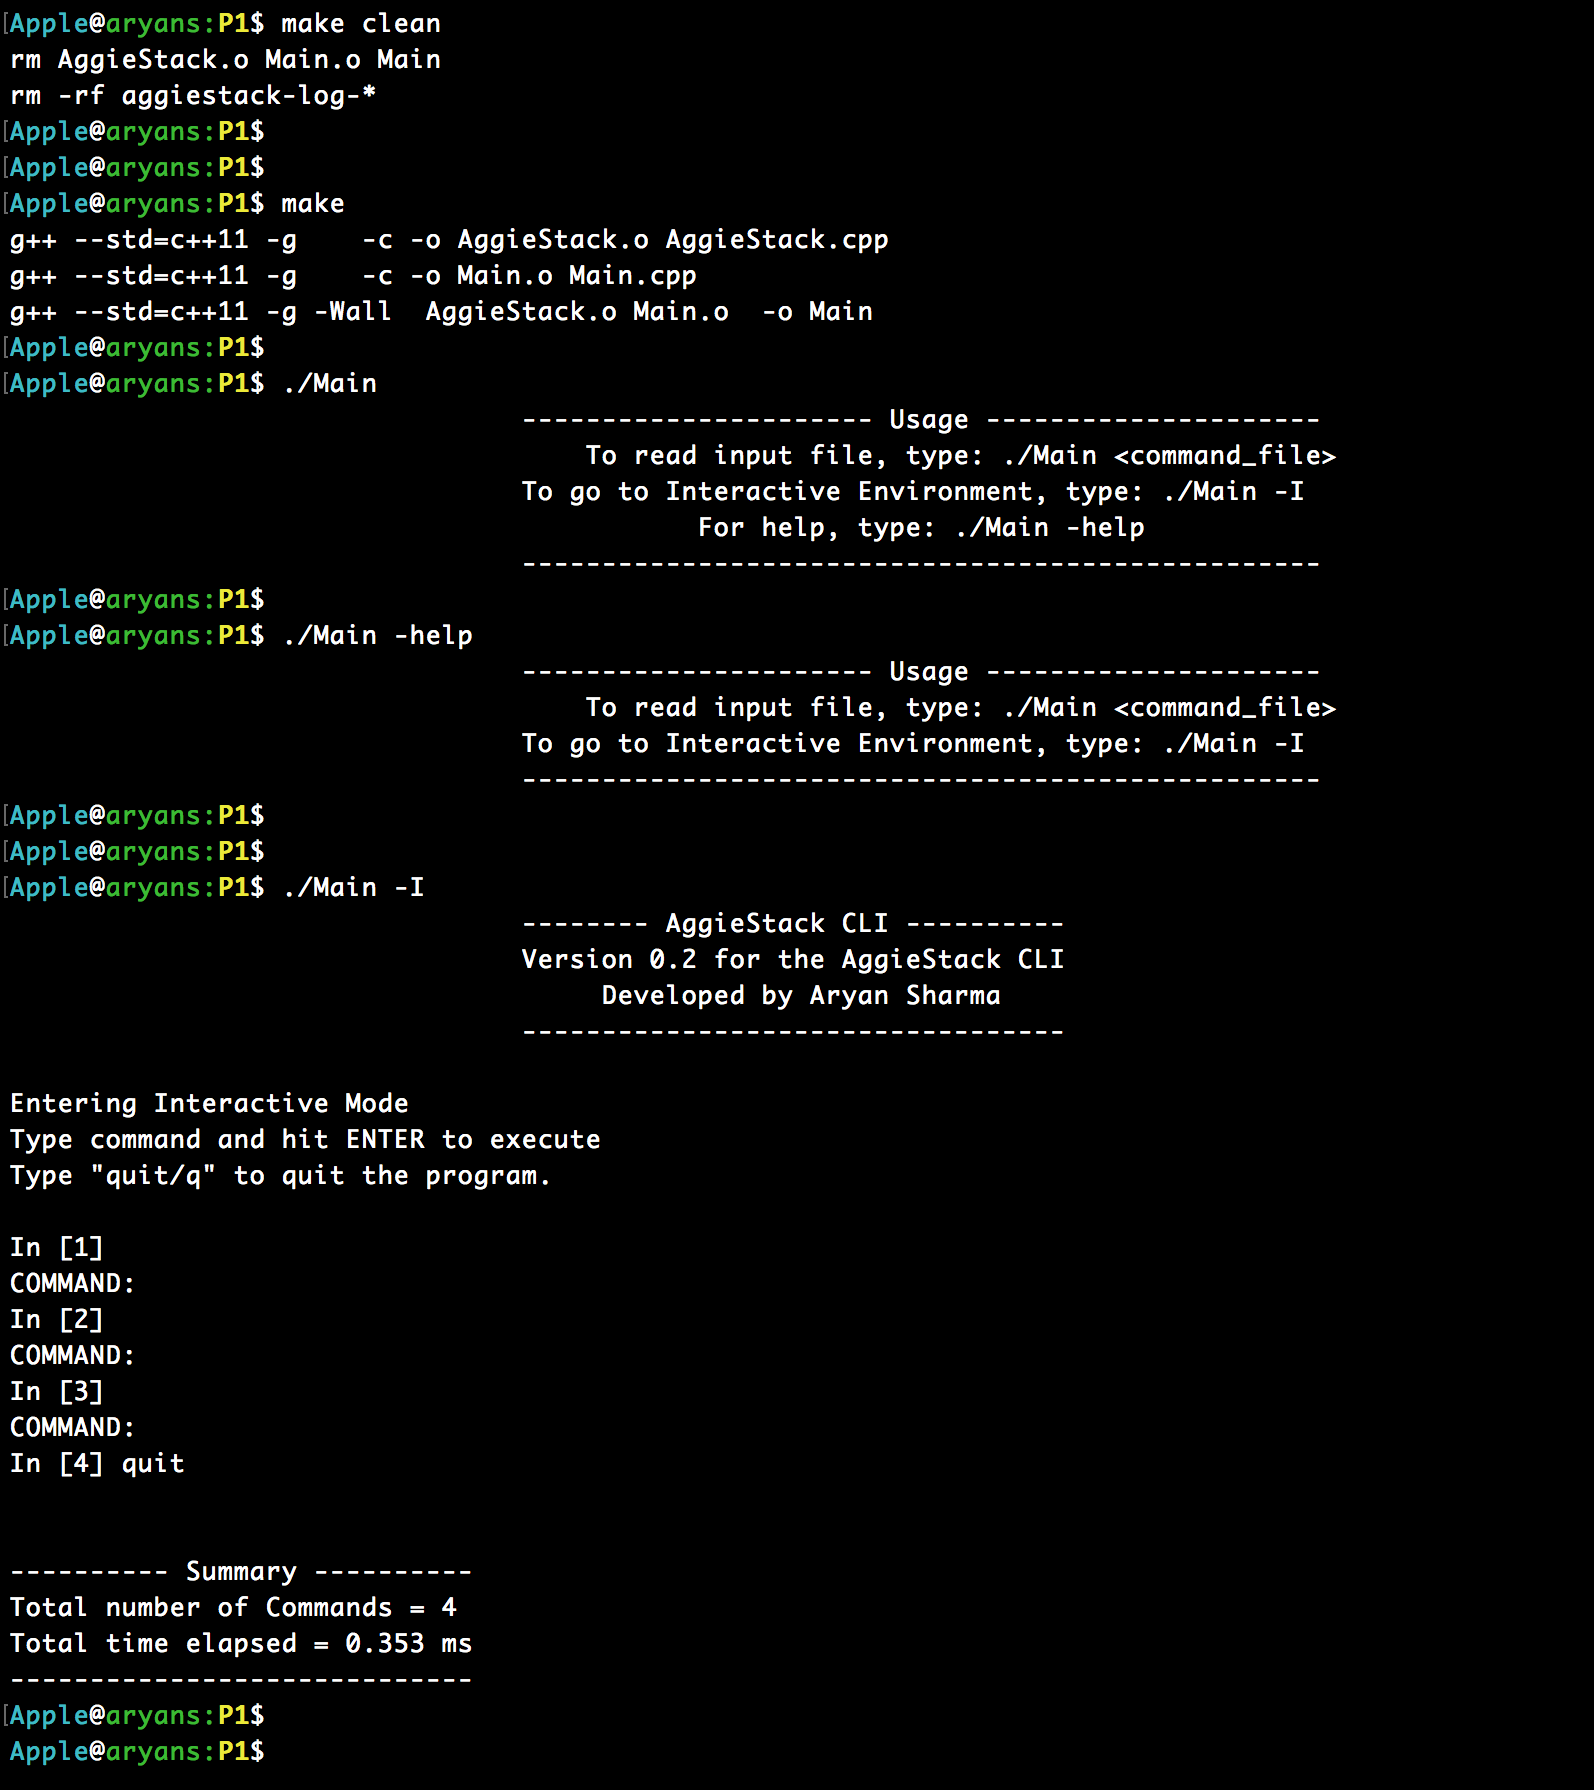
\includegraphics[width=1\textwidth]{cli1.png}
	\caption{\label{fig:data}How to run the program.}
\end{figure}

\begin{figure} [H]
	\centering
	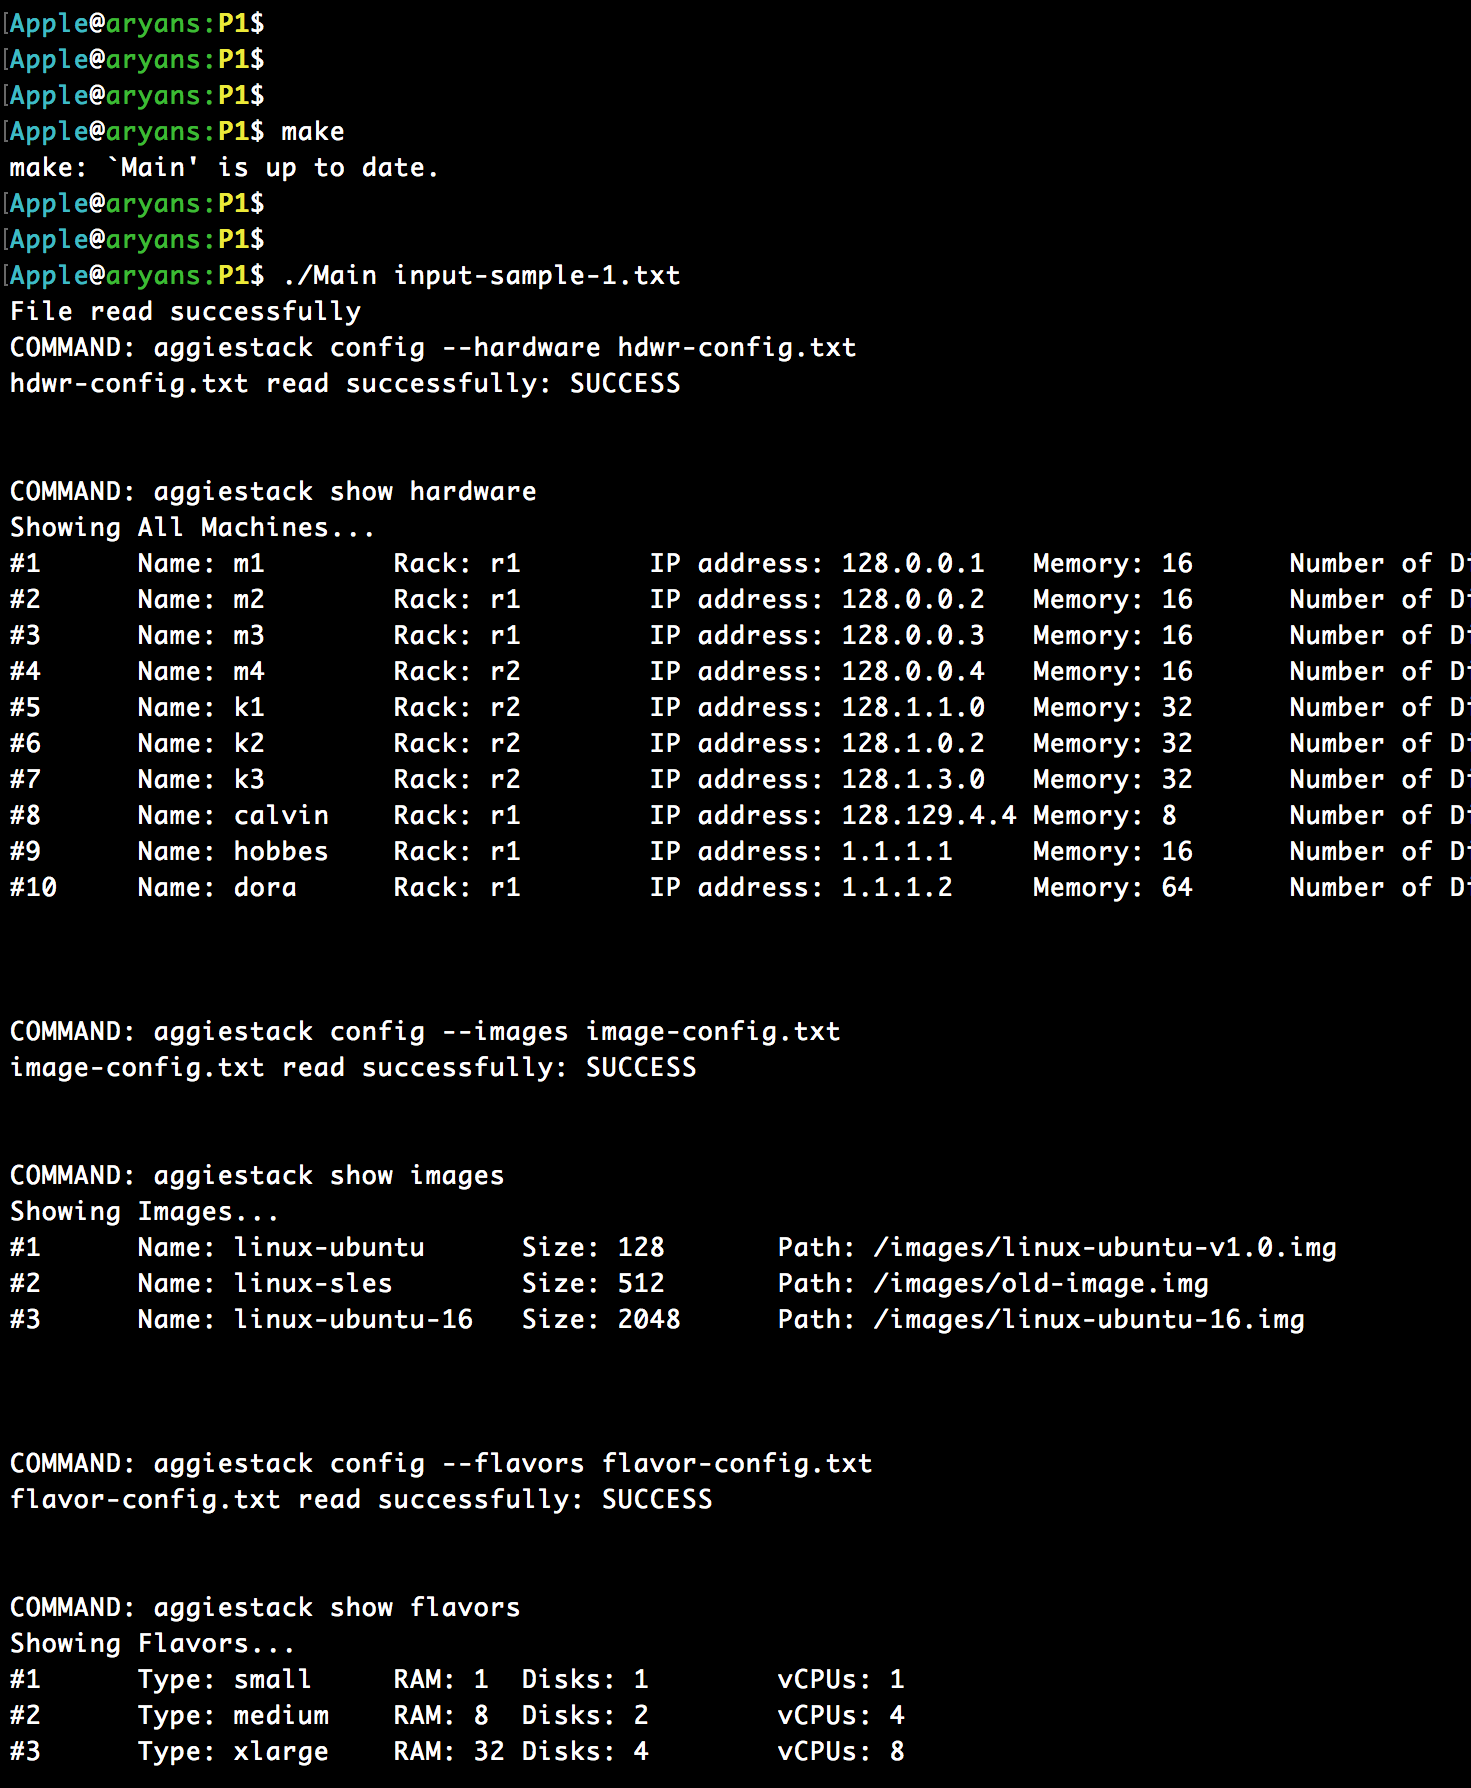
\includegraphics[width=1\textwidth]{cli2.png}
	\caption{\label{fig:data}How to run the program using an input file}
\end{figure}

The commands supported has to be entered by the user in the CLI. Some commands that are run in interactive mode has an advanced suggestions mode. There have been some hardcoded commands other than the ones the user can enter based on the sugggested syntax which can be invoked by typing \texttt{help} in the CLI. They appear in the form of option like 1, 2 etc. and may promt the user to enter some specific detail to process their requests. This has been shown in Fig. 3. You can see that by typing \texttt{help}, a list was suggested. In the Fig. 3 option \texttt{2} was selected and the file entered was \texttt{hdwr-config.txt}. As we can see the command executed was:

\vspace{1em}
\texttt{aggiestack config --hardware hdwr-config.txt}
\vspace{1em}

In the end, it generates the summary of number of commands executed in the interactive mode and the time taken to execute them. The summary can be seen in Fig. 1.

\begin{figure} [H]
	\centering
	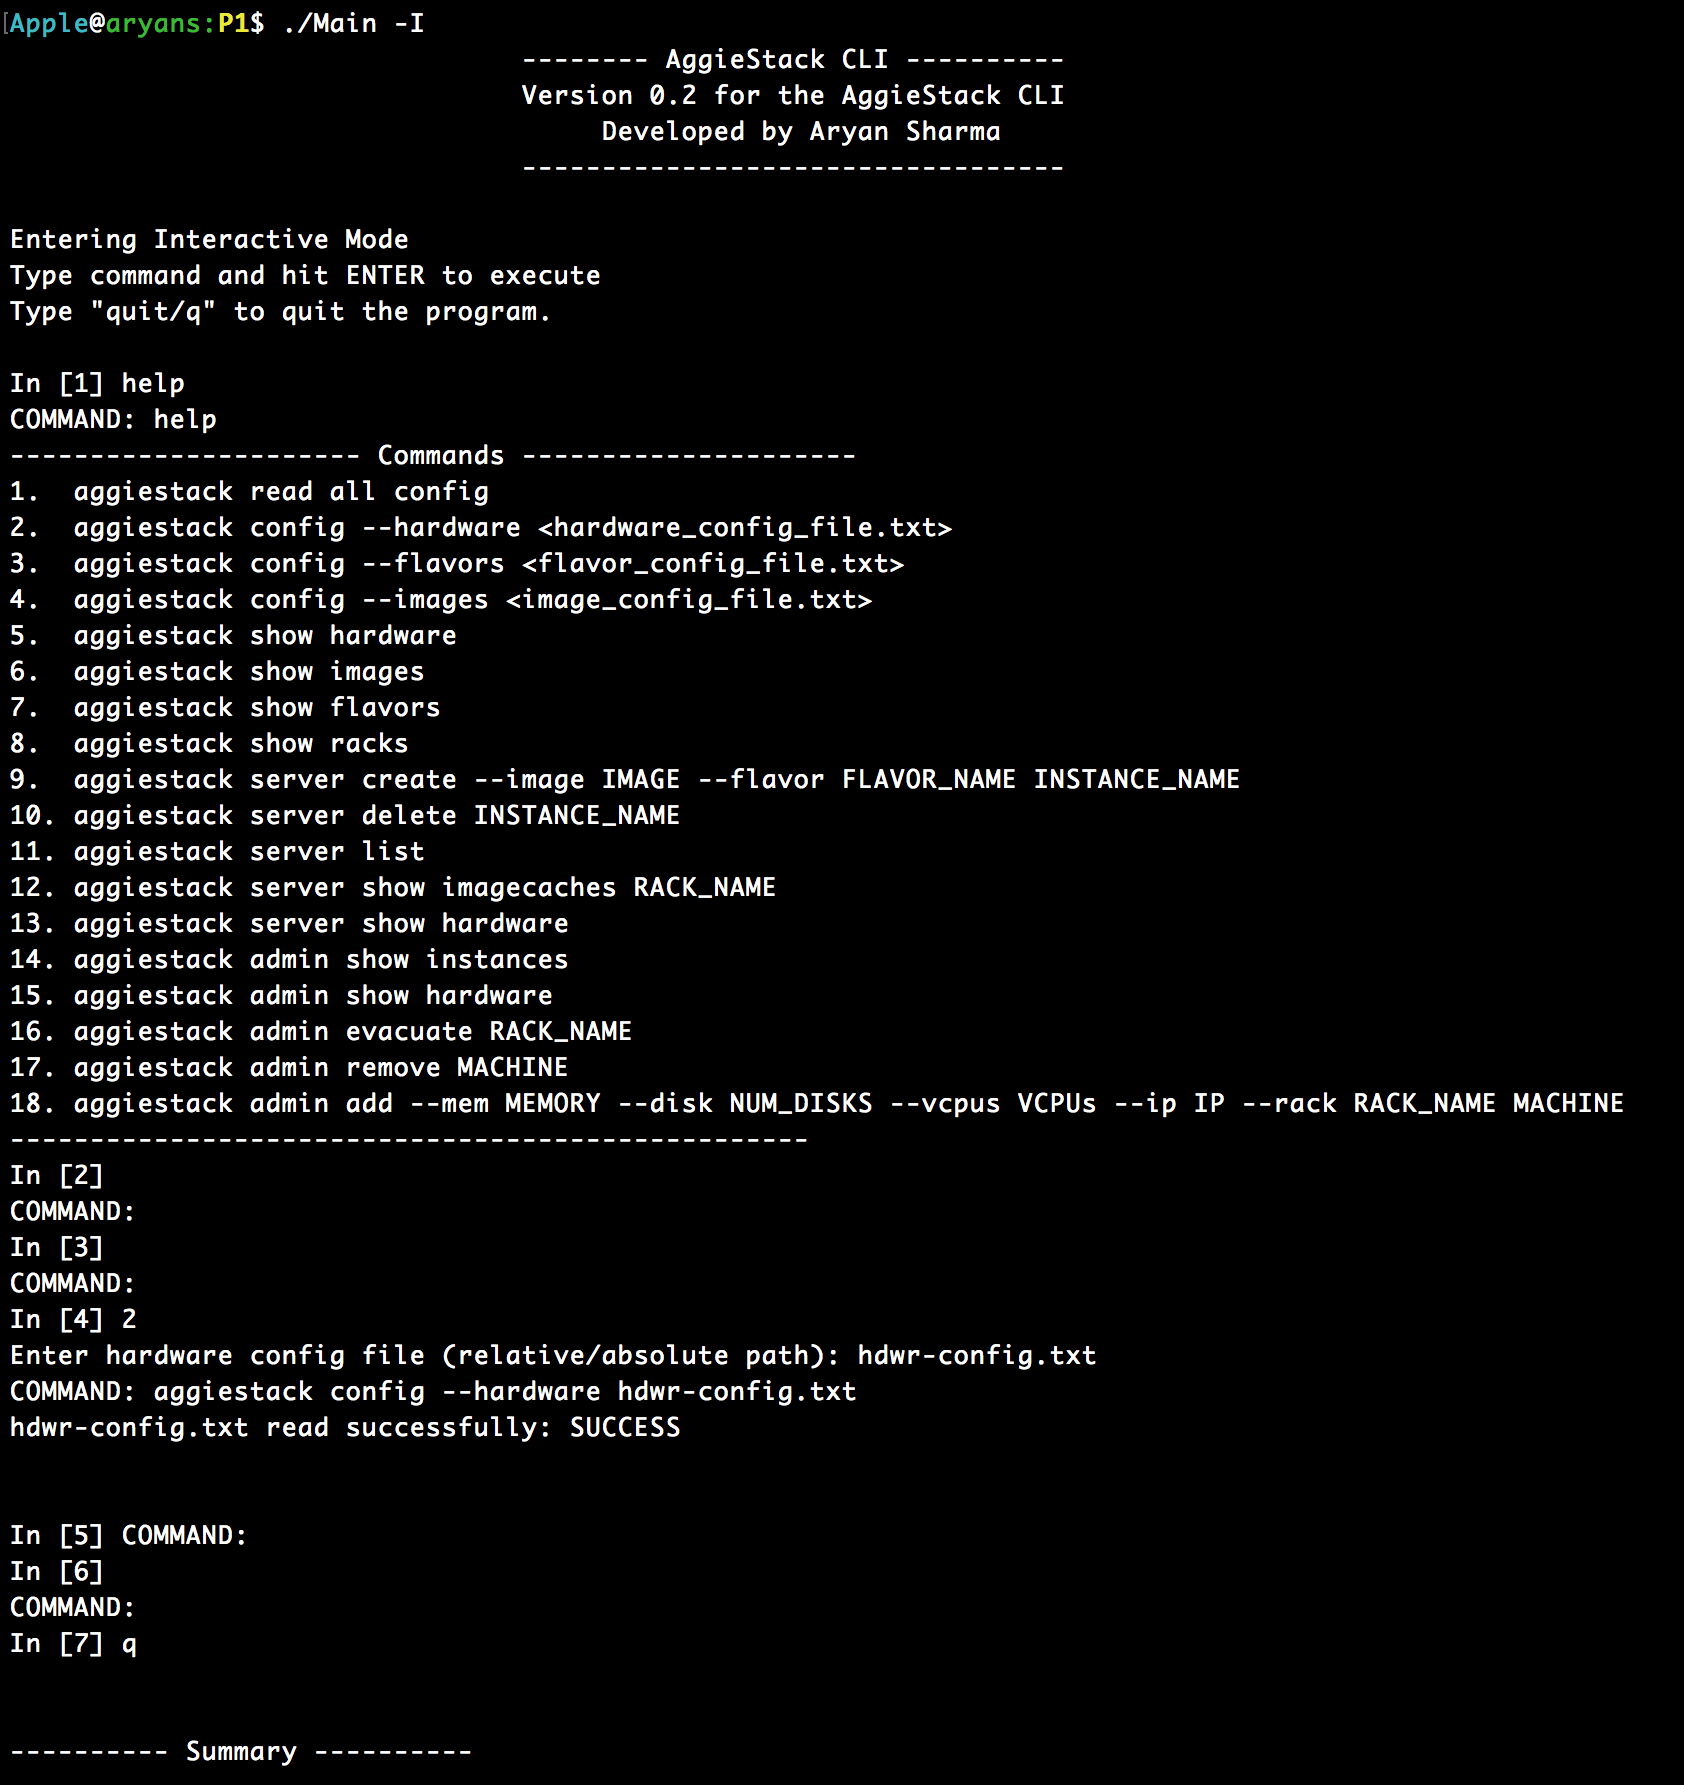
\includegraphics[width=1\textwidth]{cli3.png}
	\caption{\label{fig:data}Suggestion help mode in CLI}
\end{figure}

%\begin{table}
%	\centering
%	\begin{tabular}{|c|c|c|c|}
%		\hline
%		Table1 Size & Table2 Size & Disk I/Os & Time(ms) \\\hline
%		20 & 20 & 3593 & 266906\\
%		30 & 30 & 4212 & 387113\\
%		50 & 50 & 7457 & 552559\\
%		70 & 70 & 16195 & 1.25760e+06\\
%		100 & 100 & 22418 & 1.66148e+06\\ 
%		200 & 200 & 48057 & 3.55844e+06\\ \hline
%	\end{tabular}
%	\caption{\label{tab:widgets}Comparison of Total Time taken and Number of Disk I/Os as Relation size increases post optimization}
%\end{table}

\newpage

\section{AggieStack v0.2 Design}

The \texttt{AggieStack} has been designed as a \textbf{singleton class} which maintains a \textbf{private} list of the following: 

\begin{enumerate}
	\item Machine information
	\item Available Machines while in process
	\item Images that are available
	\item Racks that are available for use
\end{enumerate}

It has some categories of APIs which include \texttt{set} and \texttt{get}. Besides it has \texttt{read} comands to read the files, \texttt{show} comands to show the states, and some special functions like create, delete and evacuate etc. A single instance of class \texttt{AggieStack} is created and is maintained throughout the sessions to avoid any extra copy or corruption of any internal data. Also it makes the maintainance of the states quite easy. 

Other classes are that of \texttt{Machine, Image, Flavor, Rack,} and \texttt{Instance}. The hierarchy in which they are connected is as follows. The singleton instance of \texttt{AggieStack} maintains the racks and also pointers to machines that are running. The \texttt{Rack} inturn has cached images information and the list of machines that are hosted on that rack. The \texttt{Machine} on the other hand has an id to the rack on which it is hosted and can provide that information through the \texttt{AggieStack}. 

Besides, when the image, hardware and flavor config files are read, they create the \texttt{Image}, \texttt{Flavor} and as per the requirement the \texttt{Machine} objects from the class interface provided. They are maintained thorought the sessions except in the situation where they are either forced killed or have to be removed from the system. Each machines have the capability to host \texttt{Instance} class objects which are the user requested instances that they need to run. The information about the running instances are with the \texttt{Machine} themselves. 

All of the classes have in addition some special functions that help them to update their states and interact with each other. Everything has been designed such that the \texttt{AggieStack}, \texttt{Racks}, \texttt{Machine}, \texttt{Instance} hierarchy is maintained. 

\subsection{Part A design}

The part A design required the commands that create virtual servers. This was achieved by \texttt{AggieStack} by calling the Machines, deciding if they can host and then allocating the ressources to the instance. The states were internally updated and were reflected through \texttt{show} commands. If no physical machine has the required amount of ram, disks, and vcpu available, it indicates the error that it can't add the instance. The policy that was used here was to provide the instance that Machine which is found first to have available space. This was changed in part C.

\subsection{Part B design}

In this part the AggieStack admins evacuate the rack by invoking evacuate command. It migrates all the virtual machines in a server residing in the faulty rack to another rack. In case no rack has free space, it kills those instances. Also it removes the specified machine from its view of the datacenter though the remove command and add a new machine to the system so that it may receive new instances.

An interesting thing about this design was that many functions were re-used internally to make the code modular and reusable. This was kept in mind while designing the \texttt{remove\_machine, can\_host} commands.

\subsection{Part C design}

In this part the image files stored in the main storage server is copied to the storage unit for a rack, serving a number of servers in its cache. It holds copies of the image files that are made available to the servers hosted in the rack. Once the image is copied to a rack, the servers in the rack have in-rack access to the images without having to go to the external storage server. The list of cached images is maintained by every rack and is sorted based in their available memory. 

When an instance is requested, the image of the instance is searched across all racks. In case one of the rack has the image, it checks if any of it machines has the capability to host it. In case it cannot, it looks on other racks, otherwise it creates an instance there and returns. In the case that none of the racks have the cached image, it copies the image from the central storage, and creates an instance in a rack which has maximum amount of storage. The caches list is updated based on the storage of the particular rack. It's a queue kind of data structure where the oldest used image is dropped from the cache to accomodate a newer image. When all such search is exhausted, \texttt{AggieStack} return an error that it cannot host the instance due to memory issues. Please refer to the code and git commits for more details. Few of the examples have been shown in Fig. 4. 

\section{Other design decisions}

The error check has been quite strict in the command line and therfore it promts user to use the suggestion mode in the interactive mode. It logs the error in the log and prints on the console when an error happens. The \texttt{logger} function is responsible to log the results in the file \texttt{aggiestack-log.txt}. The file contains the timeline of the execution. An example is in Fig 5. 

\begin{figure}
	\centering
	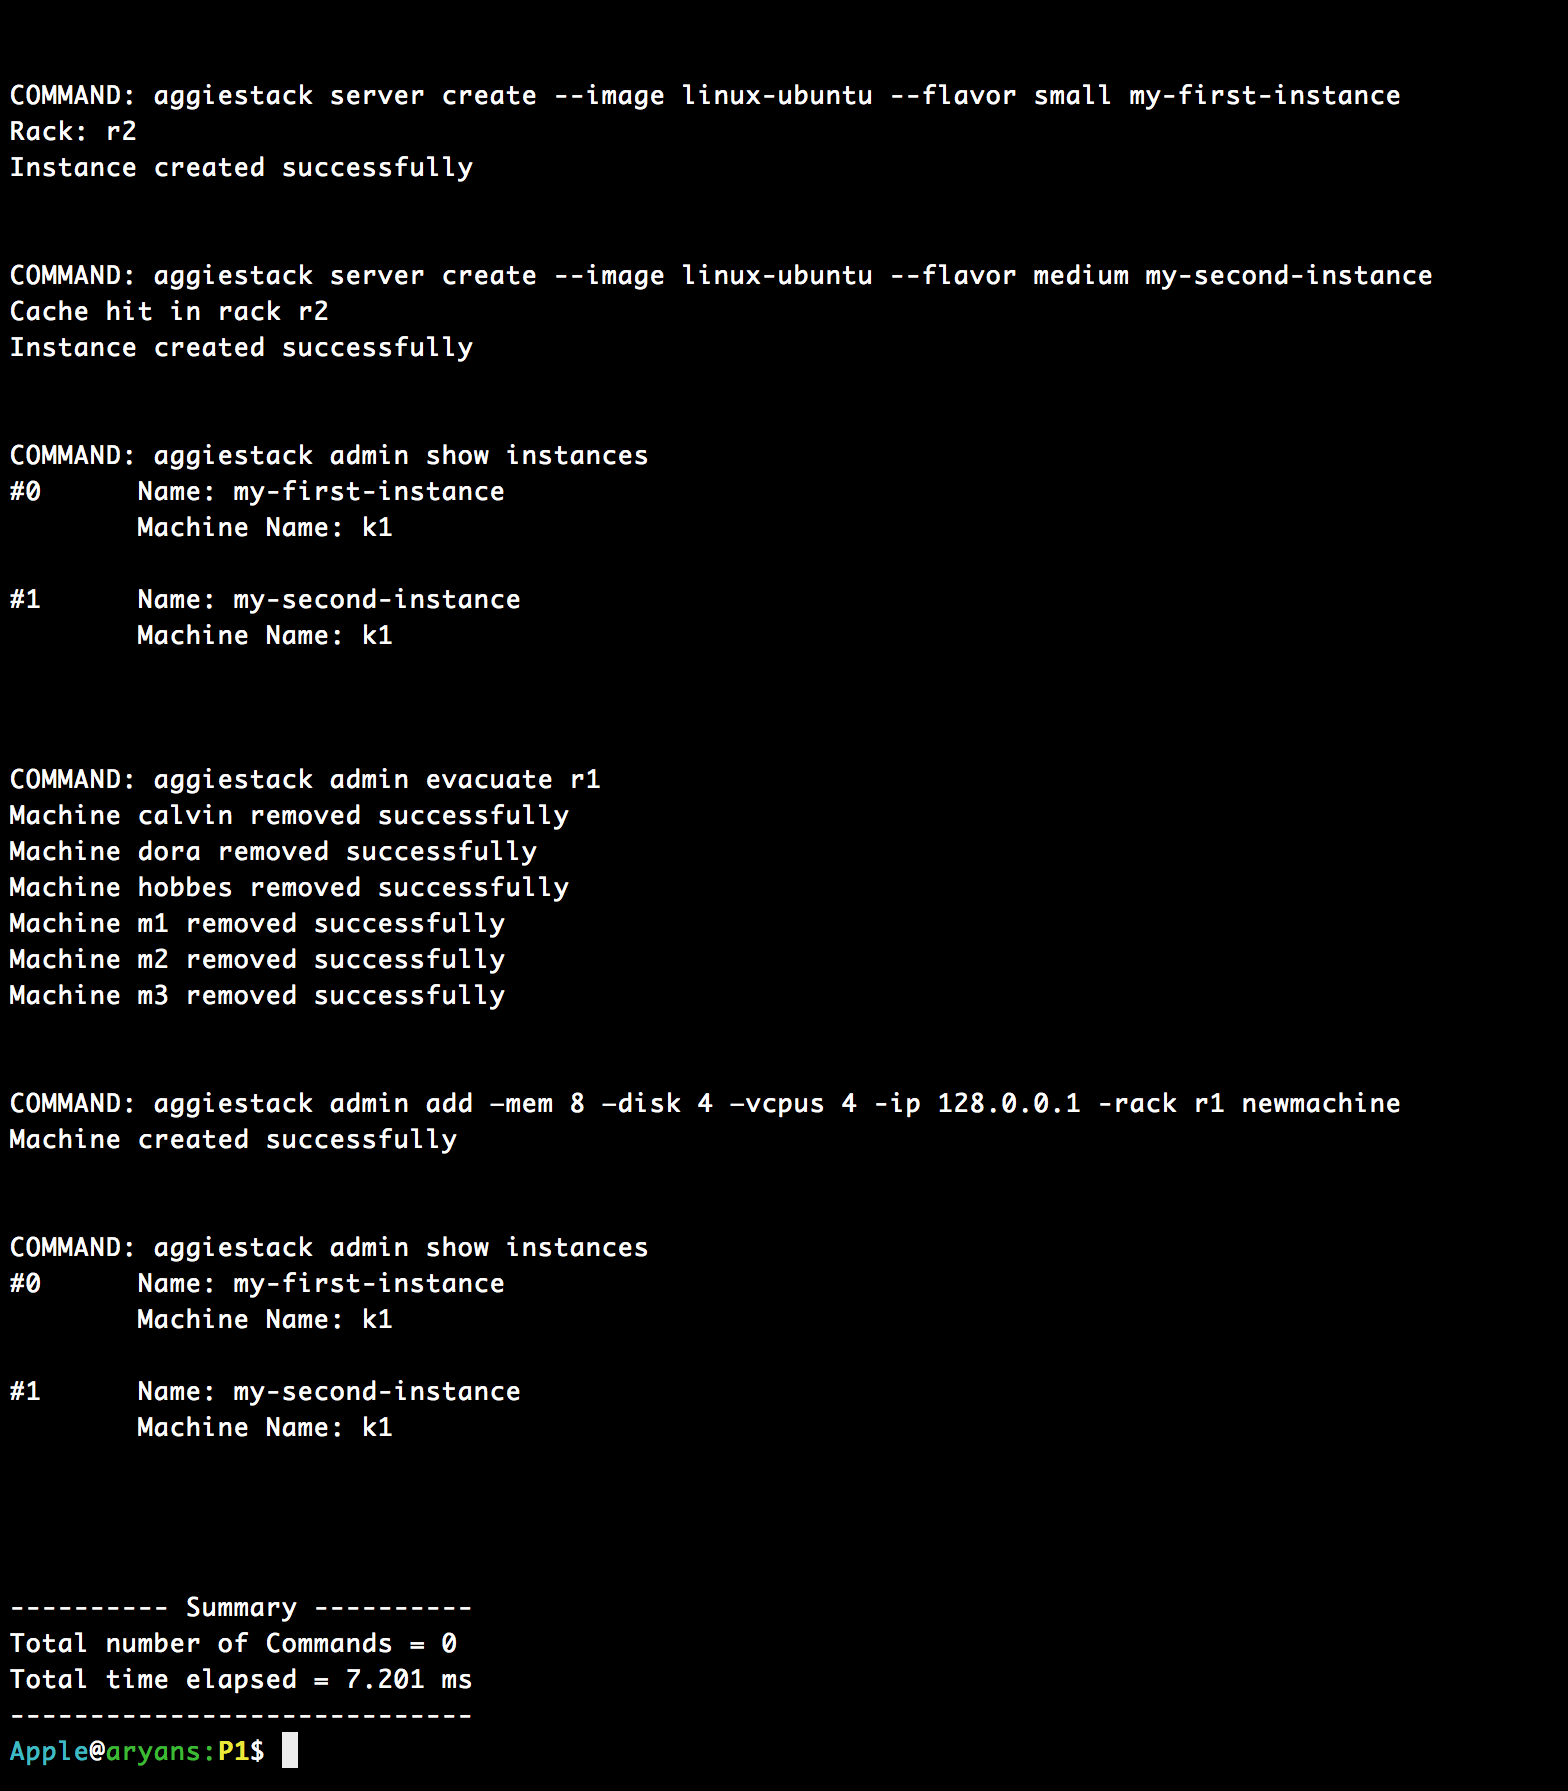
\includegraphics[width=1\textwidth]{w1.png}
	\caption{\label{fig:data}Examples}
\end{figure}

\begin{figure}
	\centering
	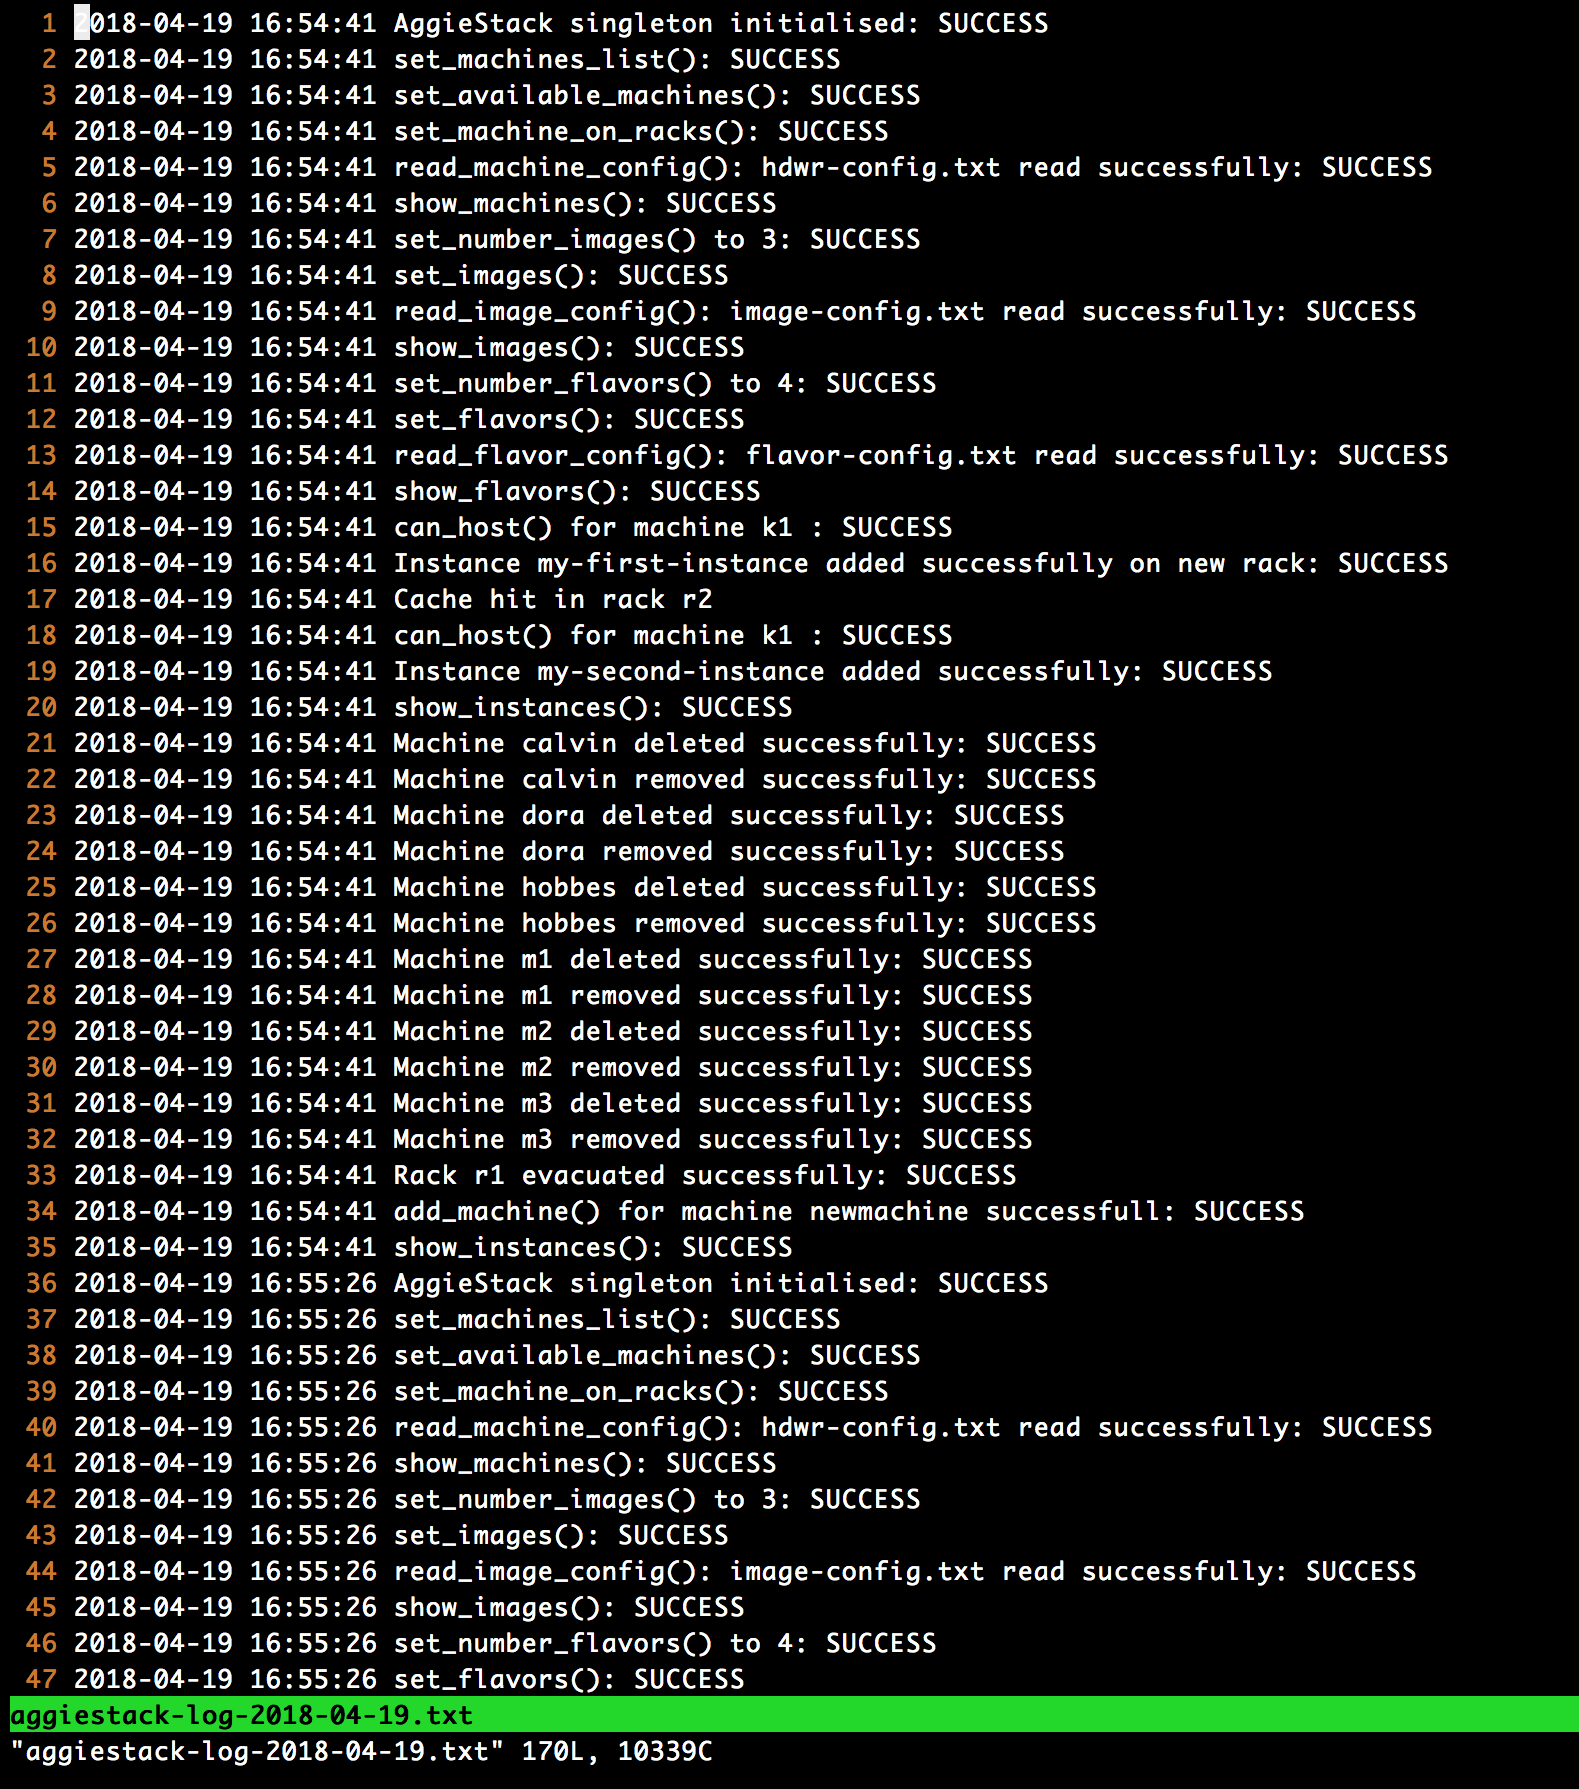
\includegraphics[width=1\textwidth]{log.png}
	\caption{\label{fig:data}Log file entry}
\end{figure}

\end{document}